% !TeX spellcheck = en_US
\section{Problem 1}

In this problem, we want to design a RBF classifier by hand. The input data are shown below. The network should produce the following output:
\[
out_{RBF} = \left\{
\begin{array}{cc}
	> 0,& \quad \text{when input vector is in the designated area}\\
	< 0,& \quad \text{otherwise}
\end{array}
\right.
\]

The designated area is consisted of two circles with centers at $\left( -1, 1.5 \right)$, $\left( 2,2 \right)$ and radius of $\rho_1 = 0.5$, $\rho_2 = 0.25$ respectively, like figure~\ref{fig:prob1_circles}.

\begin{figure}[htpb]
	\centering
	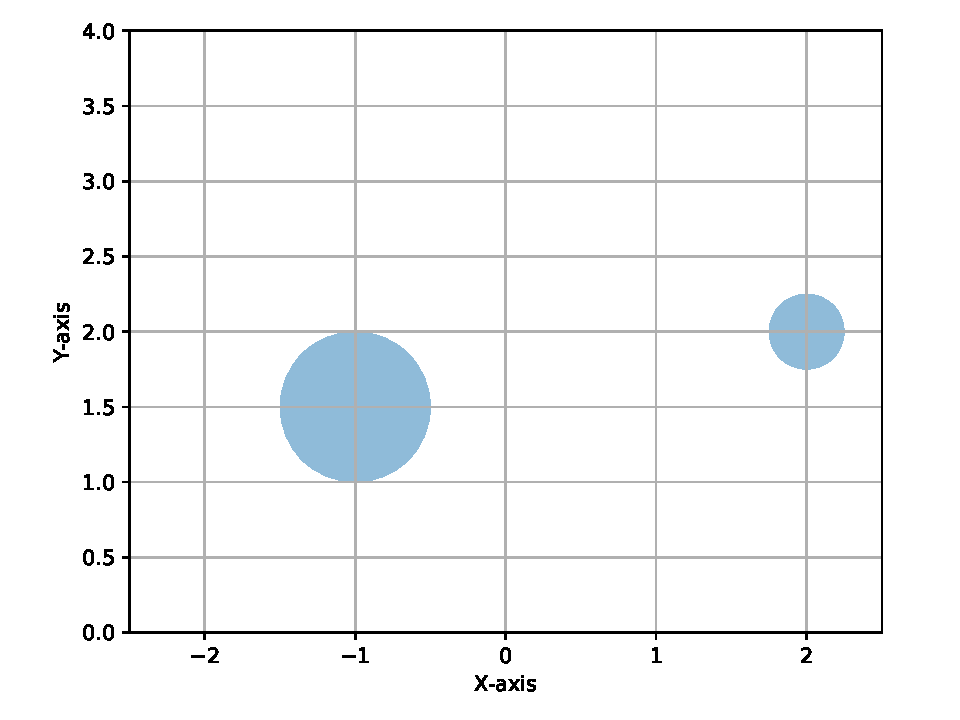
\includegraphics[width=0.5\linewidth]{../Problem 1/prob1_designated_area.pdf}
	\caption{}
	\label{fig:prob1_circles}
\end{figure}

Following the standard procedure for an RBF network, the network will have two layers. On the RBF layer, there will be two neurons, each corresponding to one of the designated regions.
As far as the output layer is concerned, there will be only a single neuron responsible for the classification output.

Moving on to some more critical parameters of the network. The centers of the RBF will be located at the same centers as the given circles, meaning at $(-1, 1.5)$ and $(-2, 2)$.
The spread ($\sigma$) needs to be chosen such that the area under the Gaussian function covers the shaded regions appropriately. 

In the absence of the exact radii of the circles, a common approach is to use the distance between the centers of the two circles to estimate the spread. The spread should typically be around the radius of the circles or slightly larger to ensure that the function covers the entire area of interest. 

The distance between the two centers can be calculated using the following equation:
\[
d = \sqrt{\left(x_2 - x_1\right)^2 + \left(y	_2 - y_1\right)^2 } = \sqrt{\left(-3\right)^2 + \left(-0.5\right)^2 } = 3.0414
\]

Since we don't want the spread to be too large to avoid overlap, we can take a fraction of this distance for each spread. If the circles are not overlapping in the classification task, we can choose the spread to be half of the distance, ensuring that each neuron's function covers its respective circle adequately.
Thus, the calculated spread is $1.52$.

Moving on to the weights of the network, we will set the weight from each RBF neuron to the output neuron to 1, assuming no overlap between the shaded regions and no need to differentiate the influence of each RBF neuron.
The weights are set to 1 to ensure that each RBF neuron's activation contributes positively and equally to the output.

Lastly, the bias of the output neuron should be set to -1, so that when neither of the RBF neurons is activated, the output neuron's activation is negative. When one or both RBF neurons are activated, the sum will be greater than 0, and the output neuron will produce a positive result.